\documentclass[12pt,a4paper]{article}
\usepackage[utf8]{inputenc}
\usepackage[english]{babel}
\usepackage{amsmath}
\usepackage{amsfonts}
\usepackage{amssymb}
\usepackage{makeidx}
\usepackage{graphicx}
\usepackage{comment}
\usepackage[maxfloats=40]{morefloats}
\usepackage[table]{xcolor}
\usepackage[left=2cm,right=2cm,top=2cm,bottom=2cm]{geometry}
\author{Alice Ledda}
\title{}
\begin{document}
\section{M  M  Github}
The whole-database tree was obtained using the SNPs only allignment.

The distance was computed from the SNP alignment using the command dna.dist in the ape package.
\begin{verbatim}
Dist<-dist.dna(all,model="N",variance=FALSE,pairwise.deletion=FALSE,as.matrix=TRUE)
\end{verbatim}


The members of each cluster where obtained using the hclust command

\begin{verbatim}
complete<-hclust(as.dist(Dist, diag=TRUE),method="complete")
groups<-cutree(complete,k=7)
\end{verbatim}

Foreach group (except the first that contained the outgroups) the entire genome of its members was collected using the following awk command

\begin{verbatim}
awk 'BEGIN{c=0}FNR==NR{a[$1]=1;next}{if(match($1,">")){s=substr($1,2,length($1)-1); 

if(a[s]==1){c=1} else {c=0}}; if(c==1)print $0}' groupN.list

 ST239_Thai_Imperial_Tong_Harris_Whole_Final.aln.fst  >groupN.fst
\end{verbatim}

An outgroup was added to make it easier the tree rooting. The outgroups for groups 2, 3 and 4 was the referece genome TW20. For group 5 was $T099\_N07\_C02$, randomly choosen from group 6. For groups 6 and 7 was $T059\_N02\_C02$, randomly choosen from group 5. We did not use TW20 in these groups as it was too far apart and we wanted something closer.

The tree was built using the following RAxML command (that produces an ML tree but also 100 bootstraps)
\begin{verbatim}
./raxmlHPC-AVX -f a -m GTRCAT -p 34235 -x 34585 -# 100 -s group6OUT.fst  

-n  group6.Boot.tre
\end{verbatim}

Then we applied ClonalFrameML
\begin{verbatim}
ClonalFrameML RAxML_bestTree.group6.Boot.tre group6OUT.fst group6.out -kappa 5
\end{verbatim}

Then we dated it it using an R script (on github is called xavierTime.R). To date we need a mutation rate per genome per year. We used 8.4 \textit{add reference}. (Genome length 3043212 bp).

To sum up most of the epi data for the dataset we created two excel files.

finaltable.xlsx contains information on the sequences, their names, the sampling date and the group they belong to. It is color-coded like the colors in the group tree.

patientDemo.xlsx contains information on the patient. It is color coded like the group tree.

Also DatingTable.csv contains important information

More epi information was used, extracted from the given files. 

The bed and sequence information is plotted in figures \ref{Group2Bed}, . On the $x$ axis there is time, on the $y $ axis information about the patients location. Each patient is identified by a color, which is the same as in the relative group tree. A solid line in the patient's color shows his/her permanence in the ICU. If the patient stayed in any other hospital ward before the permanence in the ICU or between two ICU permanences, it is shown from a dotted line in the bottom line of the graph, identified by "ward"(just because it might be important for the transmission). The bullets on top of the patient's line describe the sampling. An empty circle is drawn when the patient was sampled but the sample was negative for MRSA. A full circle is drawn when the sample was MRSA and present in the group. An empty circle with a cross is  drawn when the sample is MRSA but not present in the tree. The beds that were not used by anybody in the group are not drawn.
 

\subsection{github}

I zipped my working directory and uploaded it.

With it you will find 3 tar.gz files:

\textbf{Report} where you find the tex of this file and all the images that I included fullbsize (plus the heatmap of the distances)

\textbf{progs} the script (mainly in R, something in perl) that I used to obtain the images and run the analysis. They're messy and not commented, so you'd better leave them alone.

\textbf{ChristopheTrees} all the outputs from the tree making process. The fasta files are missing but I can upload them separately. The final version of the trees, non dated is called $groupN.out.labelled\_tree.newick$ and it is the output of ClonalFrameML

The dated trees are in the rest of the folder and are called $groupN.rootxxx.tre$. The number after root is of course where the root is according to the R script.


\section{Results}
The dataset is composed by 1020 sequences. 173 of them have been previously described in the Tong et al paper and 20 of them have already been described in the Harris et al paper and 826 samples are new. 

As for the coverage the average coverage of the samples included in the Tong et al study had an average coverage of 276, the samples in the Harris study had a coverage of 86 and the new samples had a coverage of 113, with an overall average coverage of 140 (minimum 48.5).

The dataset is composed by 277 samples from 76 patients. For each sample 1 to 27 colonies where sequenced. (see figure \ref{Nseq}) %In 93  samples at least 7 colonies were sequence, in 88 8 colonies, in 45 nine colonies, in 6 ten colonies, In 5 samples 21 colonies and in 2 samples 29 colonies.
For 182 samples we had just one colony sequenced. All the further colonies where sequenced in the last data release.

The samples belong to patients from 2 different wards, the adult ward and the infant ward.

As for the bodyparts, the vast majority of the sequences (863) come from the nose (cfr figure \ref{BodyM}). That's because all the samples with multiple sequenced colonies are nasal samples. We also have 27 axilla samples (A),36 Tracheal samples (C),  62 throat samples(T), 11 wound samples (W),2 urine samples (U) and 1 H sample (I do not know what it is, but whatever it is, it's taken from a nurse). Interestingly, patients whose samples are H and U only have that sample, so no comparison is possible. This happens also for some other bodyparts. I.e. wound for person T156. Most of the patients have samples from just one bodypart. Just very few have been sampled from a variety of bodyparts (figure \ref{BodyS})



\subsection{The groups}
Given the distances among samples in the tree (realized just from the SNPs data) we divided the dataset into 7 groups as described in Methods. We explored each group more in detail to seek answers to our questions (cfr figure \ref{tree}). The composition of the groups where highly non homogeneous as for number of samples, number of patients and bodyparts, as shown in table \ref{tab:groups}.



\begin{table}
\begin{center}
%\rowcolors{1}{white}{white}{blue}{green}{purple}{orange}{pink}{yellow}

\begin{tabular}{c*{4}{c}r}
Group            & N of & N of & body & Average & color  \\
			& sequences & people & parts & distance &    \\
\hline
2 & 65 & 25 & A,C,H,N,T,W &  & blue \\
3     & 539 & 23 & A,C,N,T,W &  & green  \\
4      & 63 & 7 & C,N,T &  &  purple  \\
5   & 34 & 9 & N,T &  & orange   \\
6    & 20 & 8 & N,T,U,W &  & pink  \\
7    & 297 & 11 & A,C,N,T,U,W &  &  yellow  \\
\end{tabular}
 \caption{Sum up of group features}
  \label{tab:groups}
\end{center}

\end{table}

\begin{comment}
\begin{table}
\begin{center}
%\rowcolors{1}{white}{white}{blue}{green}{purple}{orange}{pink}{yellow}

\begin{tabular}{c*{3}{c}}
Group            & min & mean  & max \\
			&  &	 & \\
\hline
2 &  2006.5 (2008.158) & 2008.004 (2008.236) & 2008.391\\
3     &  2006.5 ( 2008.158) &  2008.311 ( 2008.314)  &  2008.415 \\
4      & 2006.5 (2008.183) & 2008.238 (2008.266) & 2008.41   \\
5   &   2006.5 (2008.183) & 2008.224 (2008.353) & 2008.393  \\
6    &  2007.5 (2008.191) & 2008.114 (2008.223)  & 2008.262  \\
7    &  2008.24 &  2008.24  & 2008.415 \\
\end{tabular}
 \caption{Sampling times. In parenthesis the same quantities without the S samples}
  \label{tab:times2}
\end{center}
\end{table}
\end{comment}

Within and between groups distances are showed in the plots in figure \ref{dist}. These distances where computing using the SNP-only file, so many samples that in those plot have distance 0, have distance $>0$ in the trees built using the entire genome. What is clear is that the distance is multi-modal. 

Given that the groups were built, just based on genetic distance, we would have naively expected that the samples in a group would belong to patients from the same ward. We do not observe this exclusivity in any of the groups. This means that there is communication among the wards. We also have samples from the nurses, but we do not know whether they work in one ward or the other or in both.
 

\subsection{Group1}
Just the outgroup TW20.
\subsection{Group2}
65 sequences from 25 individuals. Mainly infants a part from 3 adults and 2 nurses. All the possible bodyparts except urine (figure \ref{Group2Tree})

Most of the patients in this group were in the hospital in March, T159  was in the ward in April, T230 and T234 in late April / early May and T341 was admitted and sampled at the end of May (see figure \ref{Group2Bed} )

There is essentially one main clade, all the outliers are too far to infer any transmission so we focused on the main clade (figure \ref{Group2TreePart}). 


In the main clade there are two mainly monoclonal clades. One is T009 and the other T010. They're both infants. T009 was negative on first admission but positive on readmission. T010 was negative on admission.

The H sample from nurse T056 clusters well in the middle of T009. Is it a transmission?

T159 has samples in this group and in group 3. Some colonies of the sample T159 N06 are present in both groups. T159 N04, the first positive swab, is present only in this group. One of the T159 N4 colonies is an outgroup to the T009 samples, although T009 was in hospital before T159 was admitted. The rest of the T159 positive samples are present only in group 3. 

All the colonies belonging to T010 cluster very closely together and separated from the rest of the tree.

T073 (infant) and T077 (adult) have two very closely related samples, but we have just one sample so it is hard to determine if it was a transmission. T073 was admitted a couple of days before T077 and was positive on admission while T073 was negative. T021 is genetically not far from these two, is an infant and negative on admission. Was admitted before T073, and discharged after. 

\subsection{Group3}
539 sequences from 23 people. Only five bodyparts: nose, axilla, throat, trachea and wound.

The most recent common ancestor of the samples in this group dates to early 2006. The group is easily divided into 3 subgroups whose common ancestors date to mid 2007 ($Ts2$), late 2007 ($Ts3$) and early 2008 ($Ts1$)
The subgroups are again very different in terms of number of samples and patients.

$Ts1$: $84$ samples from five individuals. Its common ancestor dates within the experiment sampling period.The samples belong mostly to two individuals: $T183$ ($48$ samples) and $T194$ (32 samples). $2$ samples from $T249$, and one sample each from $T178$ and $T159$. All of them children and were in the ICU in April. Some polychotomies, different samples of $T183$.

$Ts2$: $340$ samples from $19$ individuals. Most recent common ancestor in mid 2007.

$Ts3$: $114$ samples from 3 individuals $96$ from $T012$, $17$ from $T159$ (one of his samples is in $Ts1$) and $1$ from $T178$ who has another sample in $Ts1$. Most recent common ancestor in late 2007.


\subsection{Group4}
Group 4 has 63 sequences from 7 patients. 4 patients are adults and 2 are children (figure\ref{Group4Tree}). Patient T099 is also in group 6, so he is clearly infected with at least two different strains. This group has some tragic outcomes as one infant (T104) died and the other infant (T188) and one adult (T028) were \textit{"disc mori"} (discharged to die at home?). 


Both the infants were positive on admission while none of the adults was. While most of them were positive already on the second day at least in one bodypart, T099 stayed negative for a while, becoming positive only after one week (figure \ref{Group4Bed}).

The group is clearly divided in two main clades plus a couple of outliers. S007 is clearly an outlier.



 T188 clearly forms a clade on its own and T028 is clearly an outlier to him. This is interesting because, although they weren't in the same ward nor in the hospital at the same time they were both \textit{"disc mori"}.
 It is striking to note that T028 is the first person of this group to be admitted in the ward, and T188 is the last one.  
T188 was admitted twice to the ICU. One on April 10 to 15 (in the bed logs looks more 12 to 14) and the second on May 29. But from her sequences we see that she was infected just once and that the bacteria sequenced in the second admission are the same as in her first. In this case sequencing many colonies (on her last day of first admission and on the day of her second admission) does not add much information. Interestingly, the segregation of samples in the tree corresponds to segregation in time: although $T188$ was in the ward while the other patients where in the ICU, he was admitted to the ICU only (a week?) after the others were discharged. And in a different ward (infant instead of adult ICU).   
 
The other clade is mainly located in the adult ICU (just one sample from the infant ward), see figure \ref{Group4TreePart} and \ref{Group4BedPart}. While the samples from T071 and T092 are completely intermingled, most of the samples from T099 cluster in one clade, and only 3 of the samples are scattered around. Is it a problem with the bottleneck, like the amount/type of bacteria transmitted to T099 is different from the amount/type transmitted to T073 and T092? Or is the clade expanding in T099 more adapted to him? 

  

\subsection{Group5}
Groups 5 has 34 sequences from 9 people. Mostly from the nose (just one from the throat), see figure \ref{Group5Tree}.
The nurse T059 was sequenced on March 7th, April 25th and May 23rd (see figure \ref{Group5Beds}). All her sequences cluster. (see bullets on the blue line in figure \ref{Group5Beds})
Nurse T353 was sequenced only on May 23rd. They form a separate clade in the tree \ref{Group5Tree} Yet the most recent common ancestor of the two dates back to more than one year before, while the diversity within T059 is much more recent. The diversity within T059 looks more like multiple infections than like a single infection. Yet it is not clear why multiple infections would be all clustering together. It points to some ecological dynamics within this nurse.

The patients data is clearly clustered by data and ward (figure \ref{Group5Beds}), the infant being in the hospital more than one month before the two adults.

Patient T069 is an infant sequenced in the first half of March and discharged home on March 18th. His sequence clusters with the sequences belonging to T327 and T330, but the times are so long that we cannot safely infer a transmission.

T327 and T330 are two adults who stayed in the ICU ward in mid May. In particular T327 from May 16th to May 20th
coming directly from home and T330 from May 18th to May 20th coming from another hospital ward (S4). Considering that T327 was negative on admission  (on his first swab) on May 17th and positive on May 20th and T330 was positive on admission on May 19th we would guess that T330 infected T327. On the other hand T327 stayed in Bed 5 on May 17th, there is no data for May 18th and T330 is in the same bed on May 19 and 20. Also the only T327 sequence seems to be an ancestor to most of the T330 sequences. Still the times are very short. Both circumstances would favour T327 infecting T330.

It is relevant to point out that both patients were admitted in the afternoon/early evening but the first swab was taken the following morning. Nonetheless T327 is negative on the first swab and positive 3 days after. Does this tell us anything on the bottleneck? I mean, how probable is it that T327 got infected in the admission process and it took 3 days for the bacteria to grow and outnumber his previously negative bacteria?

It is also interesting to note that most of the T330 sequences belong to the same sample taken on May 19th and that if we had sequences just one of the 7 colonies, had we got 5, 6  or 1 the phylogeny would have been totally coherent with the epidemiology (T330 infecting T327), while the other 4 would have been incoherent. Anyway the times are so short that nothing could have been ruled out. On the other hand it would have been interesting to see what we would have seen having other 6 colonies from T327....  

It would be also interesting to understand why nobody was infected for one month and a half between the cases.

\subsection{Group6}
Group 6 is the smallest group with 20 sequences from only 8 patients. 4 of the 5 T patients are in the adult unit and one is in the infant unit (T035), see figure \ref{Group6Beds}


The infant T035 was discharged from the Pediatric ICU the day in which the first of the adults was admitted. His  sequence is far from the others. 

T095 and T107 were directly admitted to the ICU while T099 and T102 were admitted coming from another ward (but not the same ward). Finally all but T095 were negative on admission. 

As for the tree, it is rather more cartherpillary than the others \ref{Group6Tree}.

From a temporal point of view T035 should the one that has started the epidemics, the MRCA is more than one year apart. On the other hand T095 comes directly from home and is positive on admission, so it seems that she cannot have been infected in  the hospital. It is plausible that she infected both T107 and T102. All of her samples cluster together in this branch, including the only one from the throat too, which points to the fact that she was colonized by the same population both in the nose and in the throat. Yet it is interesting to note that the throat sample is more diverse than the nose ones. T099 was eventually positive just in his second admission to ICU. 
Interestingly the 4 adults had procedures related to the abdominal region.

\subsection{Group7}
297 sequences from 11 people (tree in figure \ref{Group7Tree}). All the possible bodyparts (except H that we do not know what it is and is present only once in one nurse in group 2). One big subgroup with $T126$ (see figure \ref{Group7BTree}) and one smaller subgroup without $T126$ (see figure \ref{Group7BTree}).

The smaller group is now called Group7b. There are 12 samples from 2 people, $T232$ and $T270$, both adults.
The $T270$ sample is labelled U but it should be C as it should be coming from the trachea.
Anyway, the $T232_T*$ samples and the $T270$ samples are very similar, unfortunately both were positive on admission in those bodyparts and there does not seem to be any moment in which they stay together in the same ward, although they were in the hospital at the same time for a period of a couple of days. The $T270$ was admitted and sampled days after $T232$. There is no bed share and there is a 3 days gap in their admittance to the ICU.
On the other hand $T232$ was negative on admission in the nose, and his nose samples are related to his throat samples (and to $T270$) even if they form a separate cluster.

Group7a is bigger: 285 samples belonging to 9 patients. Most of the samples belong to individual $T126$ a septic male who spent 3 months in the adult ICU overlapping with the 3-month-long study. $19$ samples belonged to $T271$, $10$ samples to $T327$ and $9$ to $T234$. Other five individuals were present with one sample each. 
All of the patients in this group were in the adults ICU except one boy who was anyway positive on admission. 
Most of the people in this group ($5$ patients) were treated for sepsi, and other two were treated for "postop", which might include sepsi??

In group 7a we find several polychotomies, and we focused on those ones to find the grups of shared bacteria.
A polychotomy in fact is no identifiable distance (below resolution?). 
$4$ polychotomies involved $T126$ and another (different ) patient, negative on admission. In these $4$ cases we are pretty sure that the other patient ($T327$, $T192$, $T234$ and $T335$) got the bacteria from $T126$ (Check dates and beds). While probably $T301$ got the bacteria from $T271$ who was positive on admission or $T249$ was positive on admission and is the same polychotomy with them (check dates and beds).
 


\subsection{Heterozygosity}

To be added...

\section{Discussion}
\subsection{the questions}
1.Would we see the same transmission patters if we had sequenced only one colony per sample?

2.Do we see different strains in different body parts?

3.If we assume that the coalescence times are real, can we say something on the bottleneck?

\subsection{T099}
T099 was admitted twice in the ICU. On the first admittance he was negative and did not become positive. On the second admittance on March 24 he was negative too. 

He gets his first positive swab on March 31. This is $T099\_N05$. We have 7 of the 9 samples in the main clade and 2 pretty distant. The next sample we have is $T099\_N07$.
Of this sample, 6 of the 9 samples cluster in the main clade, one is further apart but in the same group and 2 are in group 6, clustering with a sample coming from his wound. \textit{(a plot of the within T099 distances would be helpful)}. 

It is clear that T099 was infected in the ICU with a main clade. He was infected in the wound with a different clade, which was seen in the same day also in the nose. 

We would have needed more colonies from the wound to prove this story. Yet the fact that there are no sequences clustering with the wound ones before the wound was samples does not disprove it. The only registered patient procedures for T099 are \textit{"cut down"}, "revision" and "central line" in the ward on March 19 and 20, so there is no reason why the wound bacteria should appear only on April 5. On the other hand there is only one wound swab and it is positive, so we do not know whether before there was not the wound or it was not swabbed.

\subsection{T159}
$T159$ is an infant present in the ward from April 3rd to April 30th. She was admitted directly to the Pediatric ICU (although she was in another hospital in the region before). Her first three swabs are negative, so she probably acquired the Staph in the ward. Her samples belong to two groups, group 2 and group 3.

Interestingly her fourth and sixth samples belong to group 2, while her fifth, seventh and eighth samlples do not belong to this group.
The samples in group 3 are just three colonies. The fact that we sequenced more than one colony (8) allowed us to see a minor variant, which in the first case was 1/4 of the total sample (2 colonies), then 0, then 1/8 of the total and then disappeared.

We would think that in this case rather than multiple infection we could be seeing an infection from a mixed sample. 


\begin{figure}[!ht]
  \centering
    
2      \includegraphics[width=0.5\textwidth]{NofSeq.pdf}
  \caption{Number of sequences per patients, for the patients for which we had more than one.}\label{Nseq}
\end{figure}


\begin{figure}[!ht]
  \centering
    
      \includegraphics[width=0.9\textwidth]{bodySmall.pdf}\label{BodyS}
  \caption{The body parts for all the people for which we had more than one sample. They can be all from the same bodypart.}\label{Nseq}
\end{figure}


\begin{figure}[!ht]
  \centering
    
      \includegraphics[width=0.9\textwidth]{multiBody.pdf}
  \caption{Only patients who have samples from more than one bodypart.}\label{BodyM}
\end{figure}


\begin{figure}[!ht]
  \centering
    
      \includegraphics[width=0.9\textwidth]{groups.pdf}
  \caption{The groups on the total tree. The color code will be kept throughout the report.}\label{tree}
\end{figure}

\begin{figure}[!ht]
  \centering
    
      \includegraphics[width=0.9\textwidth]{GroupsHM.pdf}
  \caption{Patients and Groups}\label{Groups}
\end{figure}

\begin{figure}[!ht]
  \centering
    
      \includegraphics[width=0.9\textwidth]{Multigroups.pdf}
  \caption{Patients whose samples belong to different groups. }\label{GroupsS}
\end{figure}



\begin{figure}[!ht]
  \centering
    \includegraphics[width=0.3\textwidth]{Group2Dist.pdf}
      \includegraphics[width=0.3\textwidth]{Group3Dist.pdf}
       \includegraphics[width=0.3\textwidth]{Group4Dist.pdf}
        \includegraphics[width=0.3\textwidth]{Group5Dist.pdf}
         \includegraphics[width=0.3\textwidth]{Group6Dist.pdf}
          \includegraphics[width=0.3\textwidth]{Group7Dist.pdf}
        \caption{The distances for each group. In color the distances between any two sequences within the group, in grey the distances between a sequence than belonged to the group and a sequence that did not belong to the group.}\label{dist}
\end{figure}

\begin{figure}[!ht]
  \centering
    
      \includegraphics[width=0.9\textwidth]{TreeGroup2.pdf}
  \caption{Group2}\label{Group2Tree}
\end{figure}

\begin{figure}[!ht]
  \centering
    
      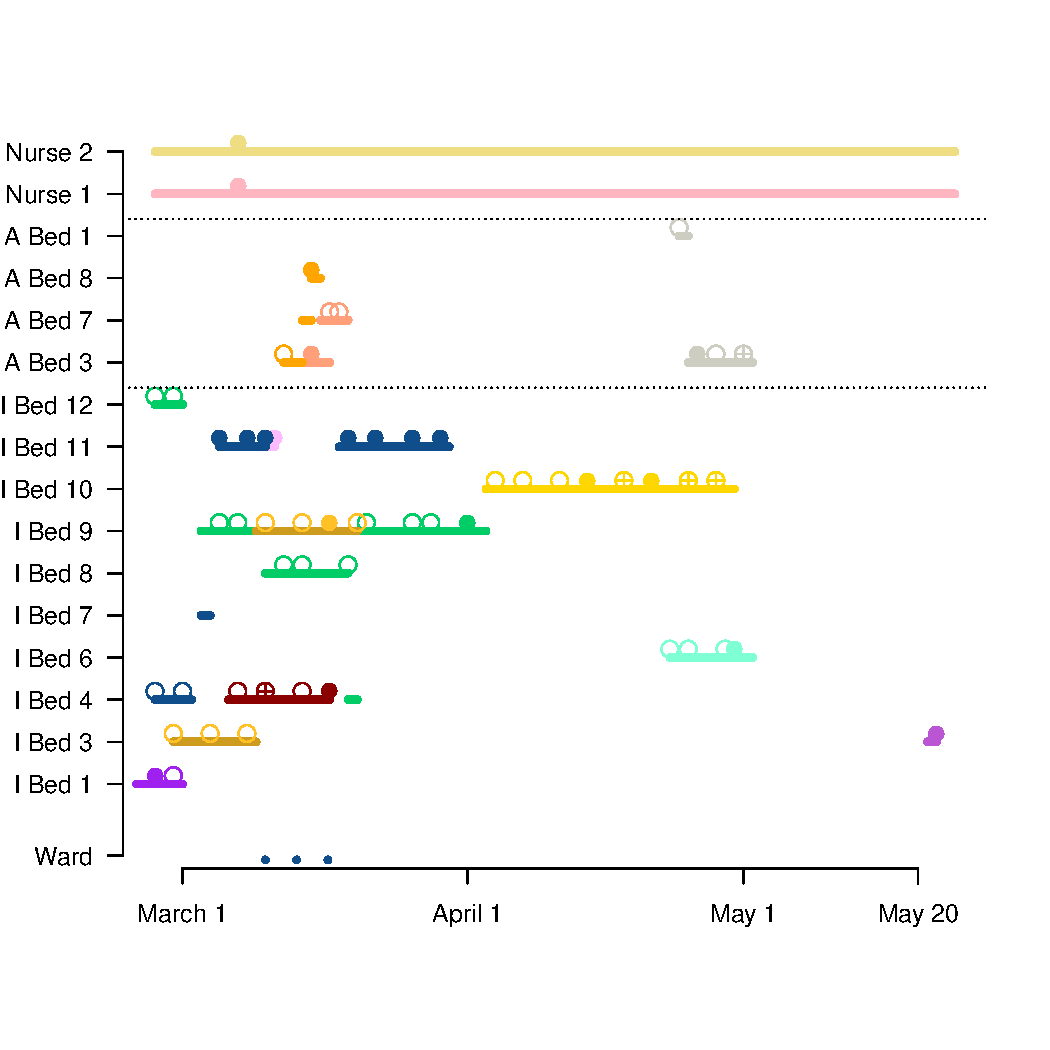
\includegraphics[width=0.9\textwidth]{Group2_Beds_2.pdf}
  \caption{Group2: summary of the Epi data.}\label{Group2Bed}
\end{figure}



\begin{figure}[!ht]
  \centering
   
      \includegraphics[width=0.9\textwidth]{TreeGroup2Part.pdf}
  \caption{Group2, detail (just one subclade)}\label{Group2TreePart}
\end{figure}
\begin{figure}[!ht]
  \centering
    
      \includegraphics[width=0.9\textwidth]{Ts1.pdf}
  \caption{Group3: first relevant clade. $84$ samples from $5$ individuals}\label{Group4Tree}
\end{figure}
\begin{figure}[!ht]
  \centering
    
      \includegraphics[width=0.9\textwidth]{Ts2.pdf}
  \caption{Group3: second relevant clade.  $340$ samples from $19$ individuals.}\label{Group4Tree}
\end{figure}
\begin{figure}[!ht]
  \centering
    
      \includegraphics[width=0.9\textwidth]{Ts3.pdf}
  \caption{Group3: third relevant clade. $114$ samples from $3$ individuals}\label{Group4Tree}
\end{figure}

\begin{figure}[!ht]
  \centering
     \includegraphics[width=0.9\textwidth]{TreeGroup4.pdf}
  \caption{Group4: tree containing all the samples belonging to the group}\label{Group4Tree}
\end{figure}

\begin{figure}[!ht]
  \centering
       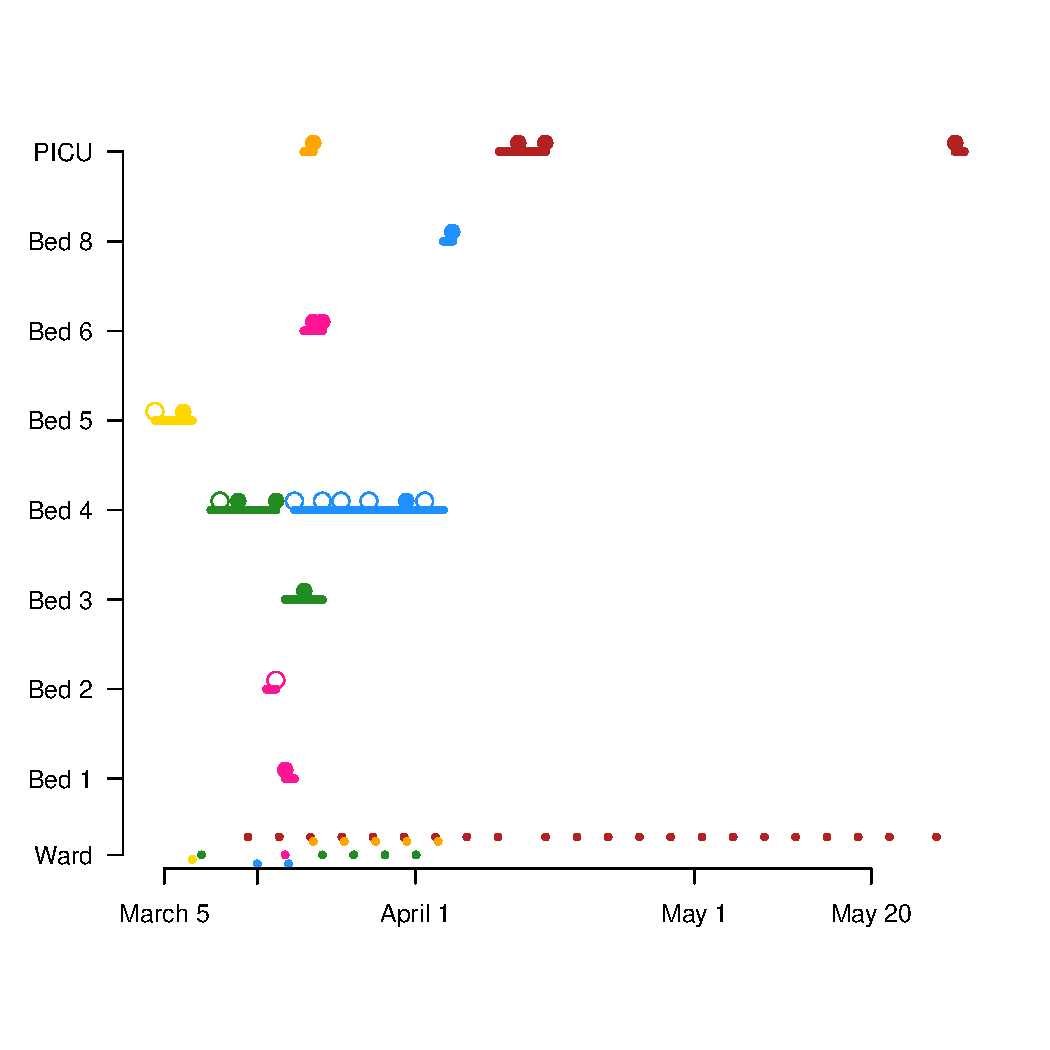
\includegraphics[width=0.9\textwidth]{Group4_Bed.pdf}
  \caption{Group4: summary of the Epi data.}\label{Group4Bed}
\end{figure}


\begin{figure}[!ht]
  \centering
     \includegraphics[width=0.9\textwidth]{group4Part.pdf}
  \caption{Group4, detail (just one subclade)}\label{Group4TreePart}
\end{figure}

\begin{figure}[!ht]
  \centering
     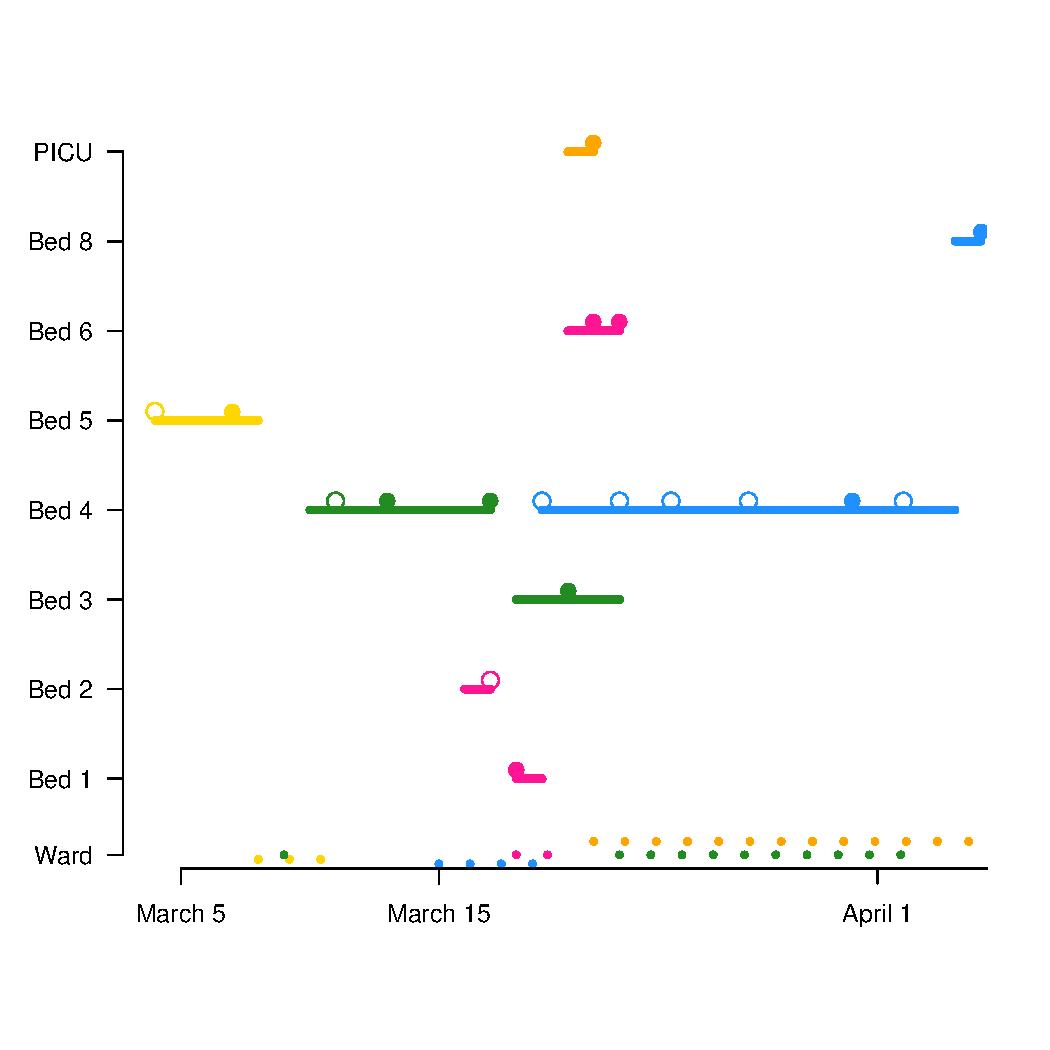
\includegraphics[width=0.9\textwidth]{Group4_beds_part.pdf}
  \caption{Group4: Epi data for samples in figure \ref{Group4TreePart} }\label{Group4BedPart}
\end{figure}

\begin{figure}[!ht]
 \centering
  \includegraphics[width=0.9\textwidth]{TreeGroup5.pdf}
  \caption{Group5: tree containing all the samples belonging to the group}\label{Group5Tree}
\end{figure}

\begin{figure}[!ht]
  \centering
  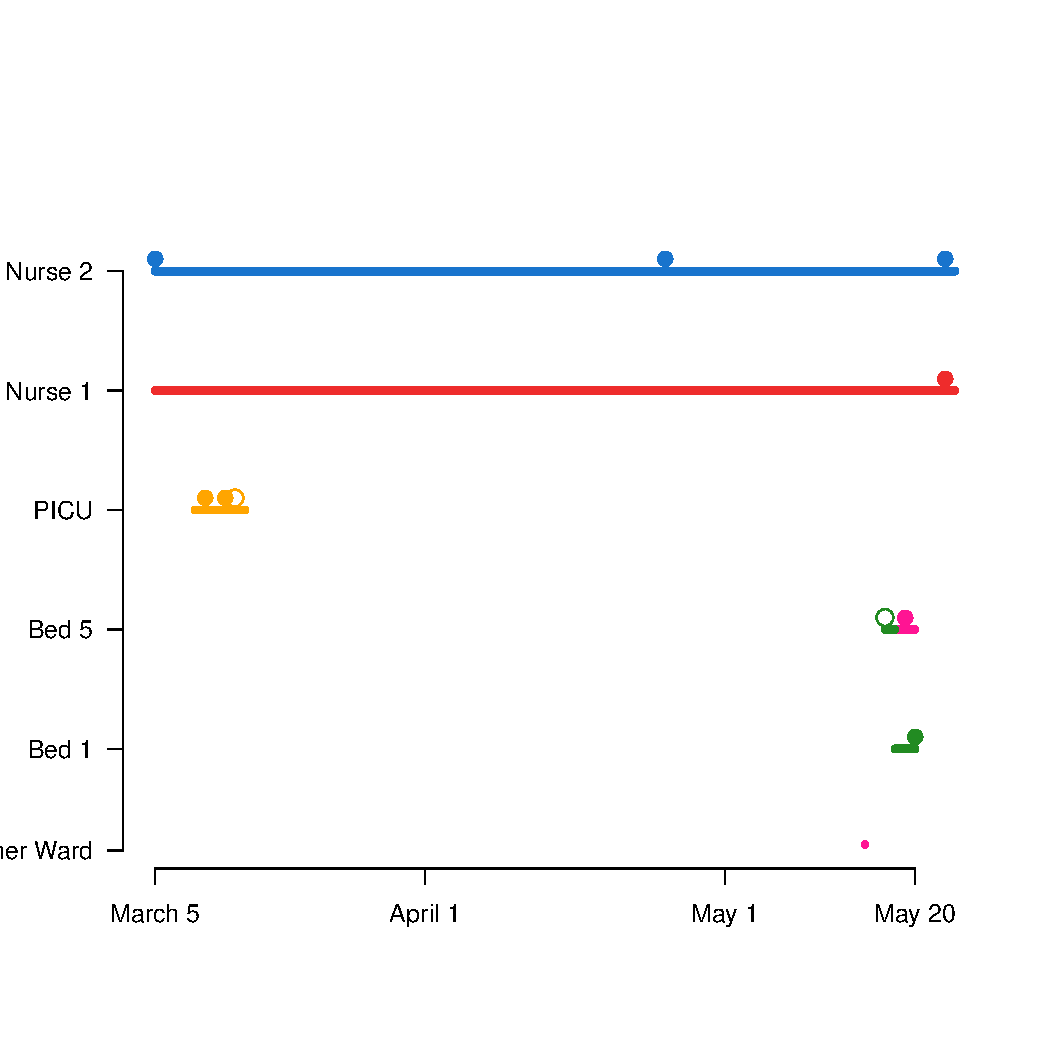
\includegraphics[width=0.9\textwidth]{Group5_Beds.pdf}
  \caption{Group5: Epi information}\label{Group5Beds}
\end{figure}

\begin{figure}[!ht]
  \centering
       \includegraphics[width=0.9\textwidth]{TreeGroup6.pdf}
  \caption{Group6: tree containing all the samples in the group}\label{Group6Tree}
\end{figure}


\begin{figure}[!ht]
  \centering
       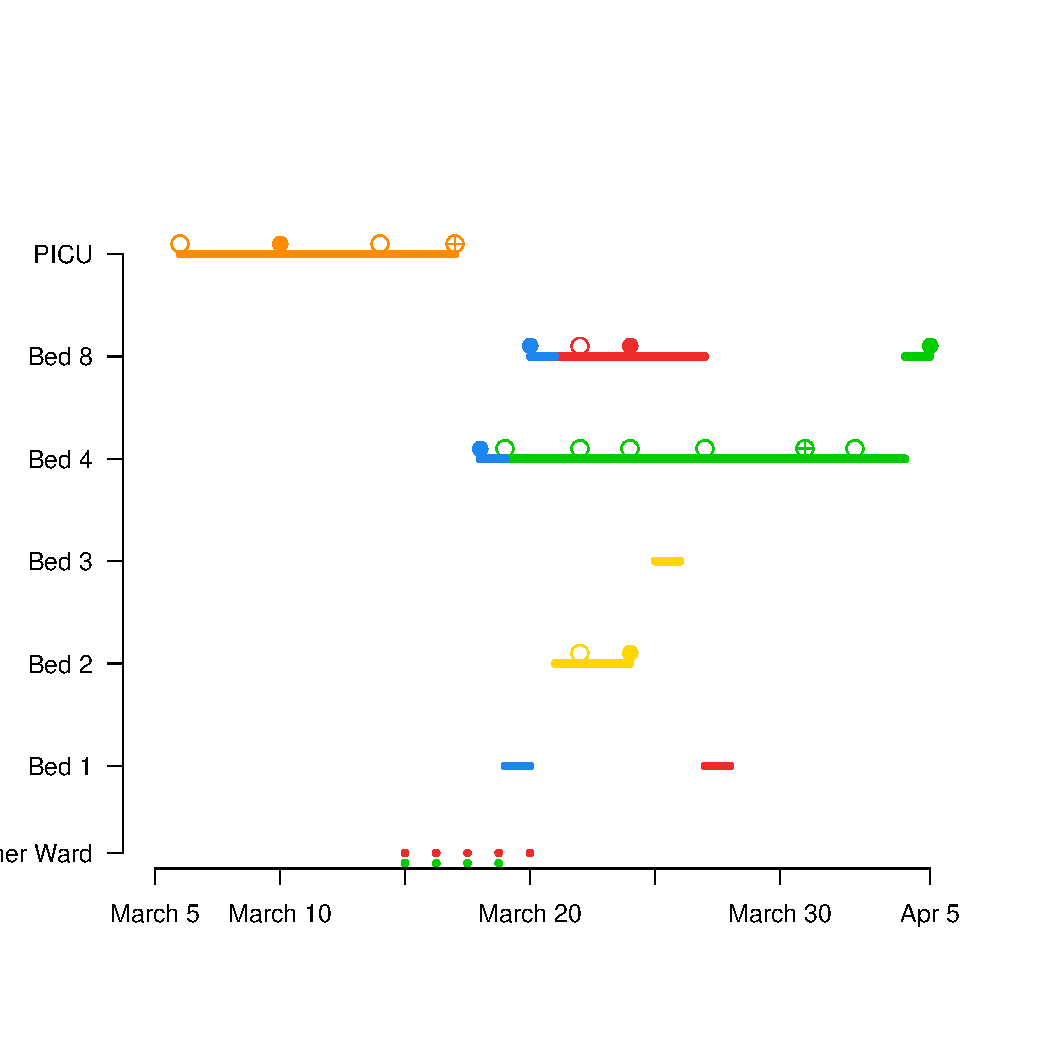
\includegraphics[width=0.9\textwidth]{Group6_Beds.pdf}
  \caption{Group6: Epi data}\label{Group6Beds}
\end{figure}

\begin{figure}[!ht]
  \centering
       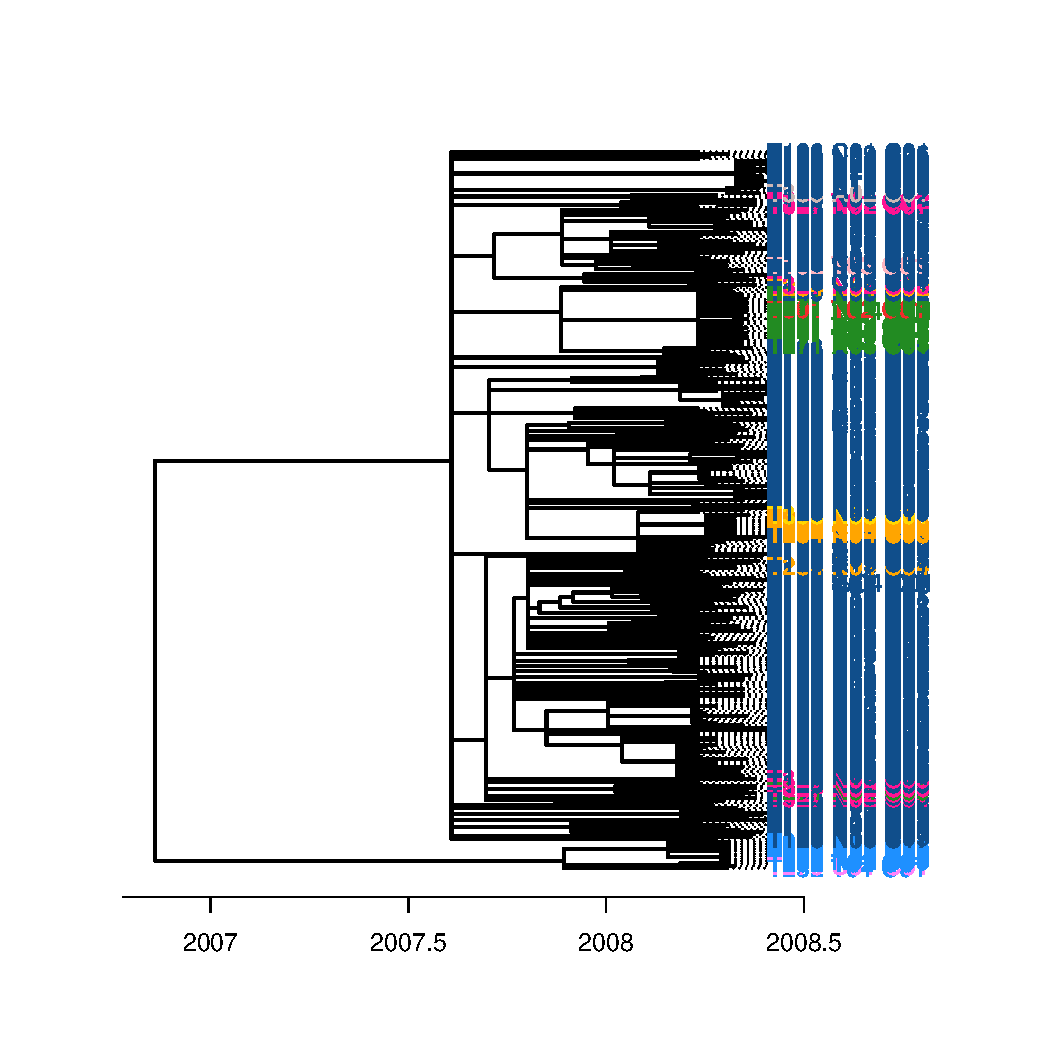
\includegraphics[width=0.9\textwidth]{group7.pdf}
  \caption{Group7: tree containing all the samples in the group}\label{Group7Tree}
\end{figure}


\begin{figure}[!ht]
  \centering
       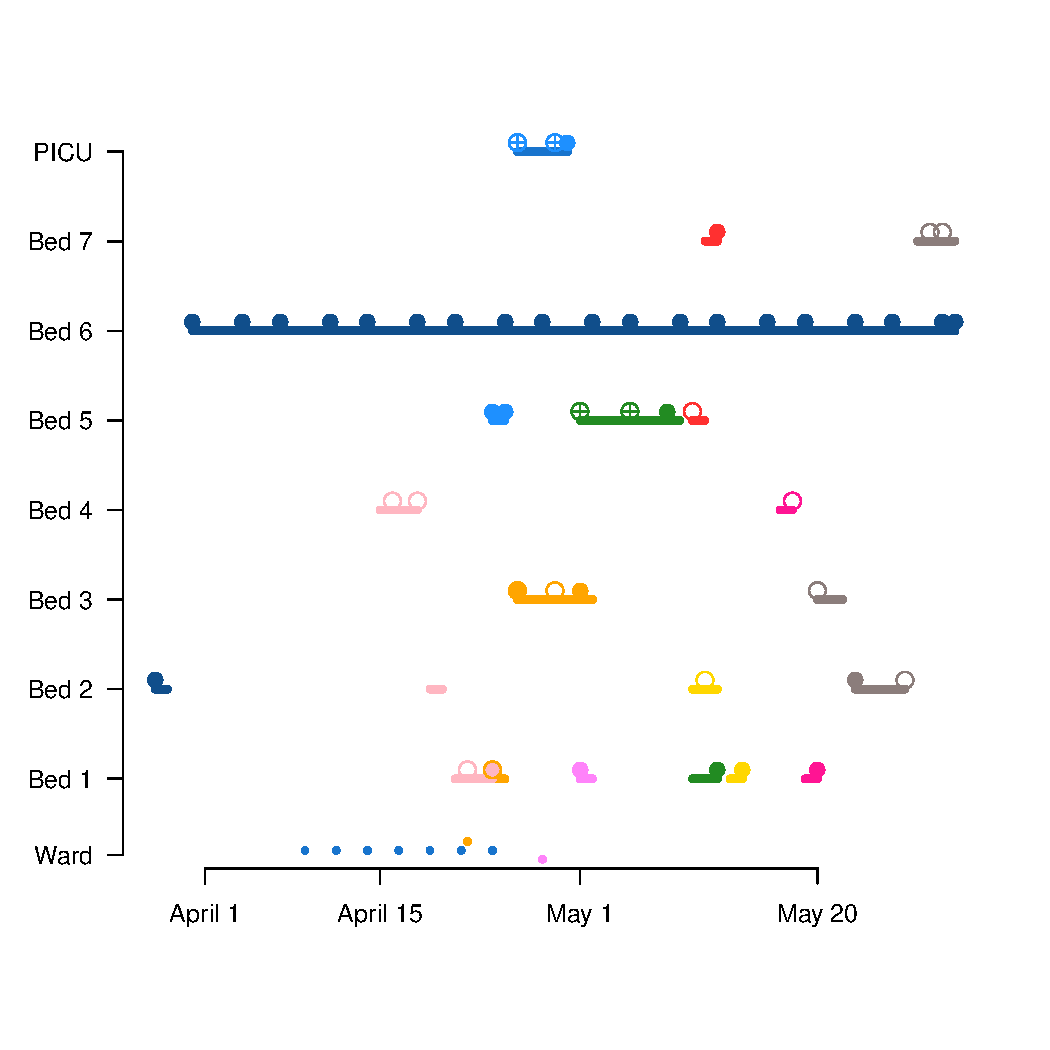
\includegraphics[width=0.9\textwidth]{Group7_Beds_2.pdf}
  \caption{Group7: Epi data}\label{Group7Beds}
\end{figure}

\begin{figure}[!ht]
  \centering
       \includegraphics[width=0.9\textwidth]{Group7a.pdf}
  \caption{Group7: detail of the more populated subclade }\label{Group7ATree}
\end{figure}

\begin{figure}[!ht]
  \centering
       \includegraphics[width=0.9\textwidth]{Group7b.pdf}
  \caption{Group7: detail of the smaller subclade}\label{Group7BTree}
\end{figure}

\end{document}
